\documentclass[border=1pt]{standalone}
\usepackage[T1]{fontenc}
\usepackage{mathptmx}
\usepackage{pgfplots}
\pgfplotsset{compat=1.18}
\usepgfplotslibrary{groupplots}
\definecolor{cA}{RGB}{31,119,180}\definecolor{cB}{RGB}{230,120,30}\definecolor{cC}{RGB}{44,160,44}
\definecolor{c1}{RGB}{31,119,180}\definecolor{c2}{RGB}{255,127,14}\definecolor{c3}{RGB}{44,160,44}
\definecolor{c4}{RGB}{214,39,40}\definecolor{c5}{RGB}{148,103,189}
\begin{document}
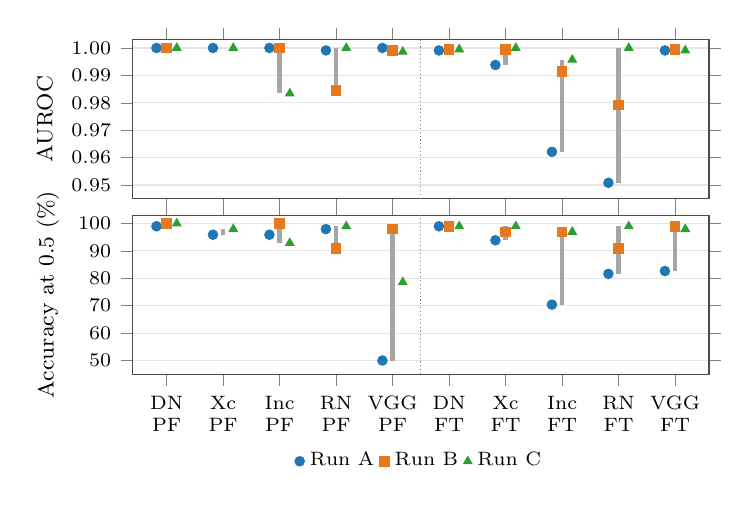
\begin{tikzpicture}
\begin{groupplot}[group style={group size=1 by 2, vertical sep=6pt},
  width=8.9cm, height=3.6cm, xmin=-0.6, xmax=9.6, xtick={0,1,2,3,4,5,6,7,8,9},
  xticklabel style={align=center, font=\scriptsize}, yticklabel style={font=\scriptsize},
  ylabel style={font=\footnotesize}, tick align=outside, axis line style={black!70},
  ymajorgrids, grid style={black!10},
  legend style={font=\scriptsize, at={(0.5,-0.42)}, anchor=north, legend columns=3, draw=none}]
\nextgroupplot[yticklabel style={/pgf/number format/fixed, /pgf/number format/fixed zerofill, /pgf/number format/precision=2}, ylabel={AUROC}, ymin=0.945, ymax=1.003, ytick={0.95,0.96,0.97,0.98,0.99,1.00}, xticklabels={}]
\draw[densely dotted, black!50] (axis cs:4.5,\pgfkeysvalueof{/pgfplots/ymin}) -- (axis cs:4.5,\pgfkeysvalueof{/pgfplots/ymax});
\draw[black!35, line width=1.6pt] (axis cs:0,1.0000) -- (axis cs:0,1.0000);
\draw[black!35, line width=1.6pt] (axis cs:1,1.0000) -- (axis cs:1,1.0000);
\draw[black!35, line width=1.6pt] (axis cs:2,0.9834) -- (axis cs:2,1.0000);
\draw[black!35, line width=1.6pt] (axis cs:3,0.9844) -- (axis cs:3,1.0000);
\draw[black!35, line width=1.6pt] (axis cs:4,0.9986) -- (axis cs:4,1.0000);
\draw[black!35, line width=1.6pt] (axis cs:5,0.9991) -- (axis cs:5,0.9995);
\draw[black!35, line width=1.6pt] (axis cs:6,0.9938) -- (axis cs:6,1.0000);
\draw[black!35, line width=1.6pt] (axis cs:7,0.9621) -- (axis cs:7,0.9957);
\draw[black!35, line width=1.6pt] (axis cs:8,0.9508) -- (axis cs:8,1.0000);
\draw[black!35, line width=1.6pt] (axis cs:9,0.9991) -- (axis cs:9,0.9995);
\addplot[only marks, mark=*, color=cA, mark size=1.7pt] coordinates {(-0.18,1.0000) (0.8200000000000001,1.0000) (1.82,1.0000) (2.82,0.9991) (3.82,1.0000) (4.82,0.9991) (5.82,0.9938) (6.82,0.9621) (7.82,0.9508) (8.82,0.9991)};
\addplot[only marks, mark=square*, color=cB, mark size=1.7pt] coordinates {(0,1.0000) (2,1.0000) (3,0.9844) (4,0.9991) (5,0.9995) (6,0.9995) (7,0.9915) (8,0.9792) (9,0.9995)};
\addplot[only marks, mark=triangle*, color=cC, mark size=1.7pt] coordinates {(0.18,1.0000) (1.18,1.0000) (2.18,0.9834) (3.18,1.0000) (4.18,0.9986) (5.18,0.9995) (6.18,1.0000) (7.18,0.9957) (8.18,1.0000) (9.18,0.9991)};
\nextgroupplot[ylabel={Accuracy at 0.5 (\%)}, ymin=45, ymax=103, ytick={50,60,70,80,90,100}, xticklabels={{DN\\PF},{Xc\\PF},{Inc\\PF},{RN\\PF},{VGG\\PF},{DN\\FT},{Xc\\FT},{Inc\\FT},{RN\\FT},{VGG\\FT}}]
\draw[densely dotted, black!50] (axis cs:4.5,\pgfkeysvalueof{/pgfplots/ymin}) -- (axis cs:4.5,\pgfkeysvalueof{/pgfplots/ymax});
\draw[black!35, line width=1.6pt] (axis cs:0,98.9796) -- (axis cs:0,100.0000);
\draw[black!35, line width=1.6pt] (axis cs:1,95.9184) -- (axis cs:1,97.9592);
\draw[black!35, line width=1.6pt] (axis cs:2,92.8571) -- (axis cs:2,100.0000);
\draw[black!35, line width=1.6pt] (axis cs:3,90.8163) -- (axis cs:3,98.9796);
\draw[black!35, line width=1.6pt] (axis cs:4,50.0000) -- (axis cs:4,97.9592);
\draw[black!35, line width=1.6pt] (axis cs:5,98.9796) -- (axis cs:5,98.9796);
\draw[black!35, line width=1.6pt] (axis cs:6,93.8776) -- (axis cs:6,98.9796);
\draw[black!35, line width=1.6pt] (axis cs:7,70.4082) -- (axis cs:7,96.9388);
\draw[black!35, line width=1.6pt] (axis cs:8,81.6327) -- (axis cs:8,98.9796);
\draw[black!35, line width=1.6pt] (axis cs:9,82.6531) -- (axis cs:9,98.9796);
\addplot[only marks, mark=*, color=cA, mark size=1.7pt] coordinates {(-0.18,98.9796) (0.8200000000000001,95.9184) (1.82,95.9184) (2.82,97.9592) (3.82,50.0000) (4.82,98.9796) (5.82,93.8776) (6.82,70.4082) (7.82,81.6327) (8.82,82.6531)};\addlegendentry{Run A}
\addplot[only marks, mark=square*, color=cB, mark size=1.7pt] coordinates {(0,100.0000) (2,100.0000) (3,90.8163) (4,97.9592) (5,98.9796) (6,96.9388) (7,96.9388) (8,90.8163) (9,98.9796)};\addlegendentry{Run B}
\addplot[only marks, mark=triangle*, color=cC, mark size=1.7pt] coordinates {(0.18,100.0000) (1.18,97.9592) (2.18,92.8571) (3.18,98.9796) (4.18,78.5714) (5.18,98.9796) (6.18,98.9796) (7.18,96.9388) (8.18,98.9796) (9.18,97.9592)};\addlegendentry{Run C}
\end{groupplot}
\end{tikzpicture}
\end{document}
